\documentclass[12pt,a4paper]{article}
\usepackage[utf8]{inputenc}
\usepackage[german]{babel}
\usepackage{amsmath}
\usepackage{amsfonts}
\usepackage{amssymb}
\usepackage{graphicx}
\usepackage{amsmath}
\author{Moritz}
\usepackage[left=2cm,right=2cm,top=2cm,bottom=2cm]{geometry}
\begin{document}
	

\title{Versuchsprotokoll}
\tableofcontents
\newpage
\section{Schallgeschwindigkeit in Gasen}
\subsection{Kalibration des Potentiometers zur Streckenmessung}
\label{section:Kalibration_Poti}
\subsubsection{Versuchsbeschreibung}
Zur Längenmessung soll ein Potentiometer eingesetzt werden. Dazu muss bei verschiedenen Auslenkungen der Widerstand R des Potentiometers gemessen werden und der entsprechenden Strecke s zugeordnet werden.\\

Für den Widerstand des Potentiometers gilt:
\begin{equation}
R = R_0(1-\frac{x}{L})
\end{equation}
Der Regelbare Widerstand ist linear in der Auslenkung x innerhalb des Potentiometers, welche wiederum linear zu der von uns verwendeten Strecke s ist.\\

Für die folgenden Versuche sind immer nur Streckendifferenzen $\Delta s$ von Interesse. Deswegen suchen wir den Umrechnungsfaktor k:
\begin{equation}
k = \frac{\Delta s}{\Delta R}
\end{equation}
Dieser entspricht offensichtlich der Steigung der Geraden durch die Messpunkte (R, s).

\subsubsection{Versuchsaufbau und - durchführung}

Vom Mikrofon aus läuft ein Seil über eine Umlenkrolle am Potentiometer, die den Widerstand reguliert. Am Ende des Seils, das hinter der Rolle nach unten hängt, befindet sich ein Gewicht, um guten Kontakt zwischen Seil und Rolle sicherzustellen. Der Widerstand R des Potentiometers wird mithilfe der Stromquellen-Box des CASSY Sensor Systems gemessen und gegen die aktuelle Position des Mikrofons aufgetragen. Als Rauschmessung für den Widerstand haben wir die Messung aus dem Versuch zur Laufzeitmessung (Kapitel \ref{section:Laufzeitmessung}) genutzt, da wir bei dieser Messung jeweils ca 20 Werte aufgenommen haben.\\

\begin{tabular}{l l l}
	
	CASSY & Kanal B & Stromquellen-Box, Rb1 0-10kOhm Momentanwert \\ 
	
	Messparameter & manuell &  7 Messungen\\ 
	
\end{tabular} 

\subsubsection{Versuchsauswertung}
Der Fehler auf die Strecken ist jeweils durch den Ablesefehler sowie den Kalibrationsfehler des Maßbands gegeben.
\begin{equation}
\sigma _{stat} = 0,05 cm / \sqrt{12} = 0,15 cm \text{\qquad} \sigma_{sys} = 0,07 cm / \sqrt{3} = 0,04 cm
\end{equation}

An diese Rohdaten wurde eine Gerade angepasst. Die Steigung dieser Geraden mit $s=k\cdot R+b$ entspricht dem gesuchten Umrechnungsfaktor $k$.\\\\
Aus der linearen Regression ergibt sich: $ k = (-15,99 \pm 0,07) \frac{cm}{k\Omega}$
\begin{center}
	\begin{tabular}{|c|c|}
		\hline
		\textbf{Strecke [$cm$]} & \textbf{Widerstand [$k\Omega$]} \\
		\hline
		10 & 2,375 \\
		\hline
		15 & 2,065 \\
		\hline
		20 & 1,765 \\
		\hline
		25 & 1,435 \\
		\hline
		30 & 1,12 \\
		\hline
		35 & 0,81 \\
		\hline
		40 & 0,505 \\
		\hline		
	\end{tabular}
\end{center}
\begin{center}
	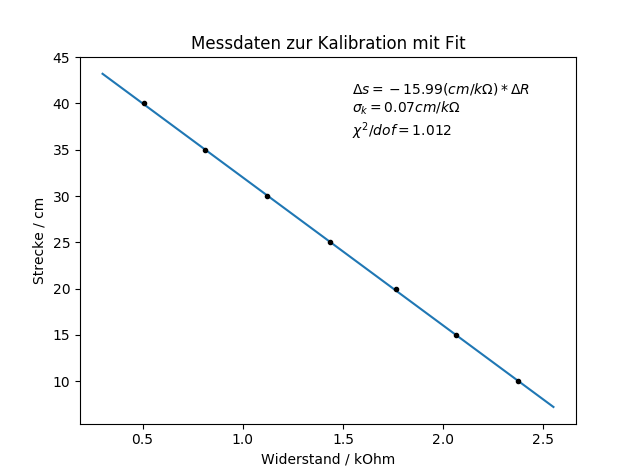
\includegraphics[width=0.7\linewidth]{kalibration_poti_fit}
\end{center}



\subsection{Laufzeitmessung}
\label{section:Laufzeitmessung}
\subsubsection{Versuchsbeschreibung}
Schallwellen breiten sich in Gasen (z.B. Luft) mit begrenzter Geschwindigkeit $v_{Schall}$ aus. Um  $v_{Schall}$ zu bestimmen, wird in diesem Versuch direkt die Zeit gemessen, die der Schall für die Ausbreitung vom Lautsprecher bis zum Mikrofon benötigt.\\
Es ist bekannt, dass in idealen Gasen gilt:
\begin{equation}
v_{Schall} = v_0 \sqrt{T/T_0} \text{\qquad mit \qquad} v_0 = \sqrt{\frac{R\cdot\kappa}{M_{mol}}T_0}
\end{equation}
Trägt man die Strecke $x$ gegen Laufzeit $t$ auf, so ergibt sich $v_{Schall}$ als Steigung der Geraden durch die Messwerte ($v=\frac{\Delta s}{\Delta t}$).

\subsubsection{Versuchsaufbau und -durchführung}

\begin{figure}
	\begin{center}
		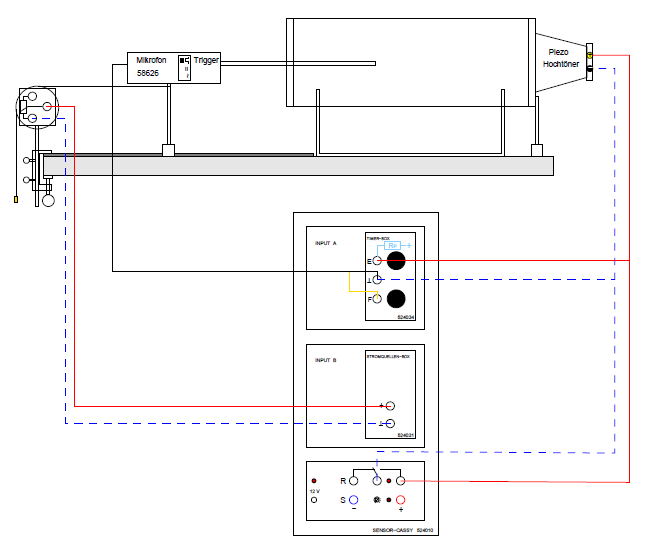
\includegraphics[width=0.7\linewidth]{aufbau_laufzeitmessung}
		\caption{CASSY Messaufbau: Laufzeit gegen Laufstrecke (Quelle: Praktikumsskript S. 38)}
		\label{pic:aufbau_laufzeit}
	\end{center}
\end{figure}


Als Lautsprecher wird ein Piezo-Hochtonlautsprecher verwendet. Dieser wird vom Relais - Schalterpaar R2/R3 des Sensor CASSY angesteuert. Diese liefern auch das Triggersignal zum Starten der Zeitmessung und das Mikrofon im Triggermodus gibt das Signal zum Beenden der Zeitmessung. Das Mikrofon steht verschiebbar auf einer Metallschiene, die mit einer Tischklemme am Ende des Tisches befestigt ist. Dort befindet sich auch ein Potentiometer (Stromquellenbox, Kanal B) mit Umlenkrolle, um Änderungen der Strecke Lautsprecher - Mikrofon aufzunehmen (siehe Kapitel \ref{section:Kalibration_Poti}). Am Ende der Metallschiene befindet sich eine Rohrhalterung mit Rohr, in dem die Messung stattfindet, um Störungen zu vermeiden. Abbildung \ref{pic:aufbau_laufzeit} zeigt den Aufbau. Außerdem wird die Lufttemperatur im Raum gemessen, um die theoretische Vorhersage für die Schallgeschwindigkeit zu ermitteln.\\\\
Um die Schallgeschwindigkeit zu berechnen, wird die Laufzeit bei unterschiedlichen Mikrofonabständen gemessen. Wir haben je Abstandseinstellung ca. 20 Messwerte aufgenommen, um den statistischen Fehler auf die Messungen zu bestimmen. Dabei ist zu beachten, dass das Potentiometer einen Abstand Mikrofon - Potentiometer liefert. Das bedeutet:
\begin{equation}
\Delta s_{Lautsprecher-Mikrofon} = - \Delta s_{Mikrofon-Poti}	
\end{equation}

\begin{tabular}{l l l}
	CASSY & Kanal A & Laufzeit Dta1 E$\rightarrow$F, 0.002s, Flanken invertiert \\
	&Relais & frac(time)<0.1\\
	Messparameter & automatisch Intervall 1s \\
	& neue Messreihe anhängen
\end{tabular}


\subsubsection{Versuchsauswertung}

Zunächst wurden die einzelnen Messreihen (Abbildung \ref{pic:messreihen_laufzeit}) auf statistische Fehler untersucht. Daraus ergab sich als Fehler für die Einzelmessungen:
\begin{equation}
\sigma _{R_{stat}} = 0,63 k\Omega \text{\qquad sowie \qquad} \sigma_{t_{stat}} = 0,29 ms
\end{equation}
Als systematischer Fehler auf die Widerstandsmessung der Stromquellen-Box haben wir ca. 1\% angenommen: 
\begin{equation}
\sigma_{R_{sys}} = 0.01 k \Omega
\end{equation}
\begin{figure}
	\begin{center}
		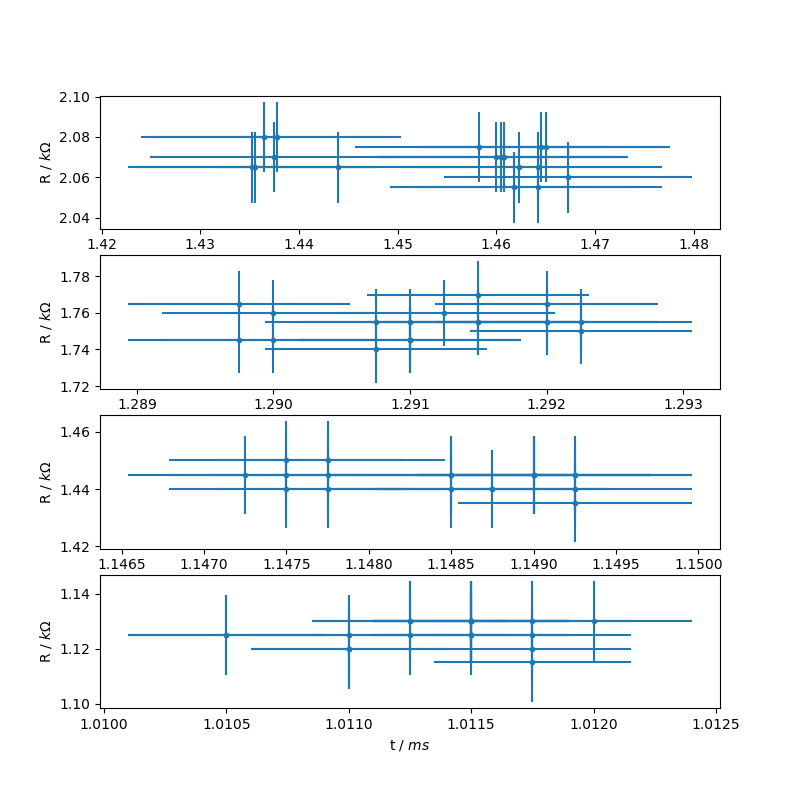
\includegraphics[width=0.75\linewidth]{messreihen_2bis5_laufzeit}
		\caption{Messreihen 2 bis 5 von insgesamt sieben Messreihen}
		\label{pic:messreihen_laufzeit}
		
		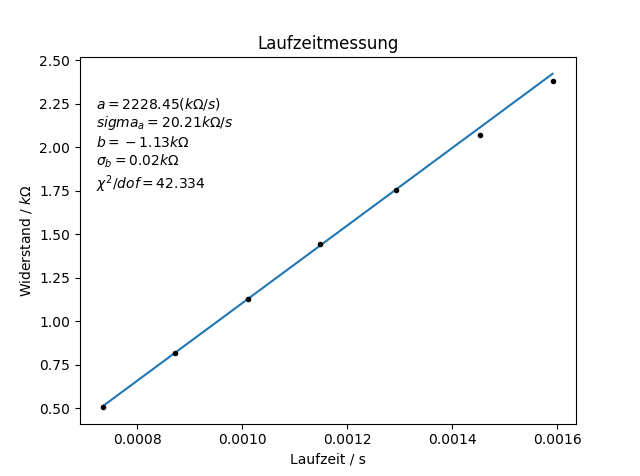
\includegraphics[width=0.7\linewidth]{fit_laufzeit}
		\caption{Mittelwerte der Messreihen mit angepasster Geraden durch die Messwerte}
		\label{pic:fit_laufzeit}
	\end{center}
\end{figure}
An alle Messreihen zusammen wurde eine Gerade angepasst (Abbildung \ref{pic:fit_laufzeit}), es ergab sich für deren Steigung:
\begin{equation}
\frac{\Delta R}{\Delta t} = (2181,55 \pm 22,77) \frac{k\Omega}{s}
\end{equation} 
Gesucht ist die Schallgeschwindigkeit $v_{Schall}$, diese ergibt sich als Steigung der Geraden an die Messwerte, wobei die Widerstände noch in Entfernungen umgerechnet werden müssen. Da nur die Steigung von Interesse ist und nicht der y-Achsenabschnitt, wurde die tatsächliche  Entfernung Lautsprecher - Mikrofon weder gemessen noch berechnet. Es gilt:

\begin{equation}
v_{Schall} = \frac{\Delta s}{\Delta t} = \frac{\Delta s}{\Delta R} \cdot \frac{\Delta R}{\Delta t} = k \frac{\Delta R}{\Delta t} = 352,11 \frac{m}{s}
\end{equation}
\begin{equation}
\sigma_{stat} = v_{Schall} \frac{\sigma _{\Delta R / \Delta t}}{\Delta R / \Delta t} = 3,64 \frac{m}{s}
\end{equation}
\begin{equation}
\sigma_{sys} = v_{Schall} \frac{\sigma _k}{k} = 1,53 \frac{m}{s}
\end{equation}

Also ergibt sich als Ergebnis des Versuchs: $v_{Messung} = (348,90 \pm 3,64 \pm 1,53) \frac{m}{s}$. \\\\
Aus der Temperaturmessung erhielten wir, dass die Raumtemperatur zu Beginn des Versuchs $T = (23,459 \pm 0,001)C = (296,609 \pm 0.001)K$ betrug.
Daraus ergibt sich eine Schallgeschwindigkeit von
\begin{equation}
v_{Theorie} =\sqrt{\frac{R\cdot\kappa}{M_mol}}\sqrt{T} = 345,1398 \frac{m}{s} \text{\qquad mit \qquad}
\sigma = 0,5 \sqrt{\frac{R\cdot\kappa}{M_mol}} \frac{\sigma_T}{\sqrt{T}} = 0,00058 \frac{m}{s}
\end{equation}
Die Abweichung der Messung von der Theorie beträgt demnach 0,73 Standardabweichungen. Die relative Unsicherheit auf  beträgt 1,48\%. Damit ist die Messung im Rahmen der angegebenen Unsicherheit nah am erwarteten Wert.
\begin{table}
	\begin{center}
		\begin{tabular}{|c|c|}
			\hline
			\textbf{Widerstand [$k\Omega$]} & \textbf{Laufzeit [$s$]} \\
			\hline
			2.3792 & 0.001591 \\
			\hline
			2.0682 & 0.001453 \\
			\hline
			1.7535 & 0.001292 \\
			\hline
			1.4435 & 0.001148 \\
			\hline
			1.126 & 0.001011 \\
			\hline
			0.8178 & 0.0008721 \\
			\hline
			0.5075 &  0.0007338 \\
			\hline
		\end{tabular}
	\end{center}
	\caption{Mittelwerte der Messreihen}
\end{table}











\section{Schallgeschwindigkeit in Gasen}

\subsection{Resonanzfrequenzen in Röhre mit fester Länge}

\subsubsection{Versuchsbeschreibung}

Ziel des Versuchs ist die Erfassung der Frequenzabhängigkeit einer stehenden Welle bei fester Resonatorlänge am schallharten Abschluss.\\
In einem geschlossenen Rohr werden Schallwellen erzeugt, welche an den Rohrenden reflektiert werden. Durch die Überlagerung von einlaufenden und reflektierten Wellen kommt es zur Ausbildung von stehenden Wellen. Dabei gibt es Orte an denen der Schalldruck für alle Zeiten verschwindet (Knoten). Für diesen Versuch sind die Druckbäuche von Interesse, für welche die Druckamplitude maximal ist.\\
Bei fester Rohrlänge erhält man für die Resonanzfrequenzen, bei denen der Druck maximal ist den Zusammenhang:

\begin{equation}
f_n=\frac{n\cdot v}{2L}
\end{equation}

mit der Rohrlänge $L$, der Ordnung der Resonanz $n$ der Schallgeschwindigkeit\footnote{Eigentlich Phasengeschwindigkeit, ohne Dispersion stimmt diese mit der Schallgeschwindigkeit überein.}  $v$ und der Frequenz $f_n$.
Misst man nun die Frequenz bei bekannter Länge L, so kann damit die Schallgeschwindigkeit bestimmt werden.\\

\subsubsection{Versuchsaufbau und Durchführung}

\begin{figure}
	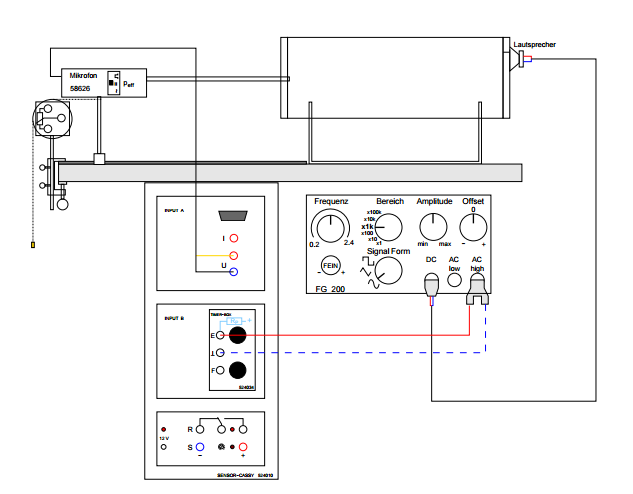
\includegraphics[width=\linewidth]{aufbau}
	\caption[Aufbau]{Schematischer Versuchsaufbau (Quelle: Praktikumsskript S.40)}
	\label{fig:aufbseite40}
\end{figure}



Die Röhre wird auf beiden Seiten verschlossen. An der einen Seite befindet sich ein Lautsprecher, auf der anderen das Mikrofon welches im Effektivwertmodus betrieben wird.
Mit dem BNC-Lemo-Adapter wird der Lautsprecher an den niederohmigen DC-Ausgang des Funktionsgenerators angeschlossen. Der rechte Hochpegel AC-Ausgang wird mittels der CASSY Timer-Box an den Kanal B des Sensor-CASSY angeschlossen. Das Mikrofon ist mit dem Kanal A des CASSY verbunden. Ein schematischer Aufbau findet sich in Abb.  \ref{fig:aufbseite40}.\\
Für den Funktionsgenerator wurden für die Signalform eine Sinusschwingung mit Offset null und mittiger Amplitude im Bereich $0.2-2.4 kHz$ gewählt.\\

Für den Kanal A des CASSY wurde der Messbereich der Spannung zu $0-3V$ gewählt mit Nullpunkt links und gemittelt über $1s$.
Die Timer-Box an Kanal B ist auf den Bereich bis $5000Hz$ mit Torzeit $1s$ eingestellt. Die Messung selbst wird manuell durchgeführt.\\

Zunächst wird die Länge des Rohres mit einem Maßband gemessen.
Die Frequenz des erzeugten Tons wird fortwährend erhöht und dabei manuell Spannungsmesswerte des Mikrofons aufgenommen. Die Lage der Resonanzfrequenzen kann bereits vorher abgeschätzt werden. Diese Bereiche werden mit dem Funktionsgenerator sehr kleinschrittig durchlaufen um die schmalen Resonanzen möglichst gut zu erfassen.

\subsubsection{Versuchsauswertung}
\begin{figure}
	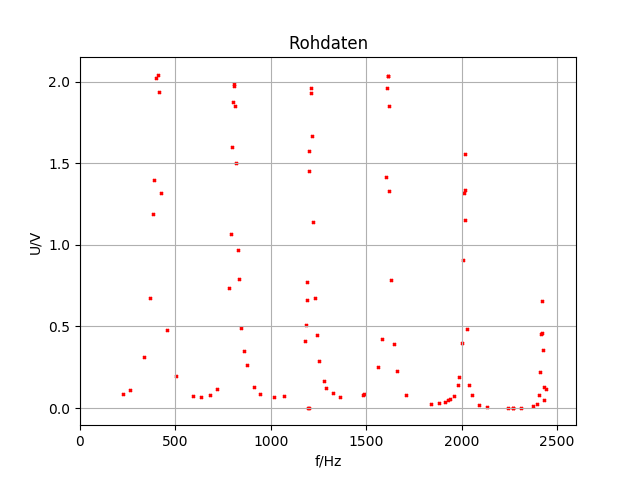
\includegraphics[width=\linewidth]{rohres}
	\caption{Rohdaten der Resonanzmessung}
	\label{fig:rohresonanz}
\end{figure}
Die Länge wurde mit einem Maßband der Güteklasse II zu $L=42.8cm$ gemessen. Der statistische Ablesefehler beträgt $\sigma_{L,stat.}=0.3mm$, der systematische Fehler ergibt sich zu $\sigma_{L,syst.}=0.7mm$.

Zur Bestimmung der Frequenzpeaks wurde der gesamte Messbereich symmetrisch um die erste Abschätzung der Peaks in je sechs Intervalle mit einer Gesamtlänge von $240Hz$ ($f_n \pm 120Hz$) unterteilt. Diese Intervalle wurden in $10Hz$ Schritten zehnmal verkleinert, einmal mit festgehaltenem linken Rand, einmal mit festgehaltenem rechten Rand und einmal mit Verkleinerung beider Ränder. Dabei wurde jedes mal mittels der peak-Funktion der Praktikumsbibliothek die Position der Peaks bestimmt. Aus den so entstehenden 33 Werten für jede Resonanzfrequenz wurde Mittelwert und Standardabweichung gebildet. Damit ergeben sich dann die Resonanzfrequenzen die Werte in Tab. \ref{resonanztabelle}.\\

\begin{table}
	\begin{center}
		
		\begin{tabular}{|c|c|c|}
			
			\hline 
			$n$ & $f_n$[Hz] & $\sigma_{f_n}$[Hz] \\ 
			\hline 
			1 & 404,11 & 1.47 \\ 
			\hline 
			2 & 809,60 &  1.72 \\ 
			\hline 
			3 & 1209.22 & 1.29 \\ 
			\hline 
			4 & 1613.86 & 1.32 \\ 
			\hline 
			5 &   2013.32 & 1.29 \\ 
			\hline 
			6 & 2420.10 &     0.96 \\ 
			\hline
		\end{tabular}
		\caption{Resonanzfrequenzen und Unsicherheiten}
		\label{resonanztabelle}
	\end{center}
\end{table} 

Eine lineare Regression ($f(n)=a \cdot n+b$) ergibt $a=402.94 Hz$, $\sigma_a=0.30 Hz$, $\b=1.40 Hz$ und $\sigma_b=1.32 Hz$. Eine grafische Darstellung des Ergebnisses findet sich in Abb. \ref{fig:resonanzregression}.  Bei sechs Datenpunkten und zwei zu bestimmenden Parametern erhält man für diese Anpassung $\chi^2/ndof=2.13$, was dafür spricht, dass mit obigem Vorgehen die Fehler etwas zu klein geschätzt wurden.\\

\begin{figure}
	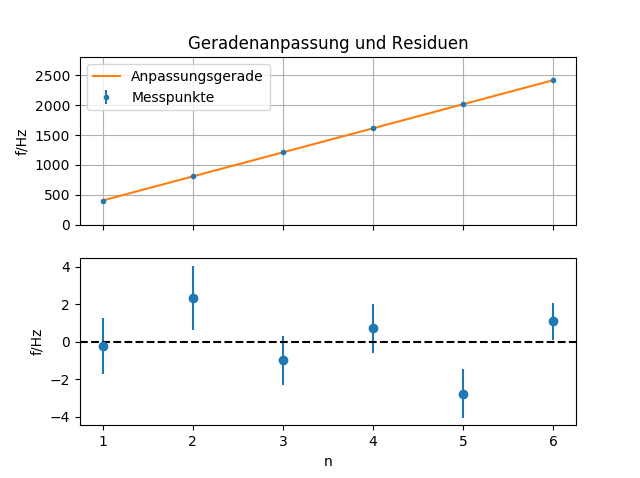
\includegraphics[width=\linewidth]{fitplot}
	\caption[Auswertung Resonanz]{Messpunkte und Regressionsgerade (oben) und
		Residuen (unten).}
	\label{fig:resonanzregression}
\end{figure}


Aus $a=\frac{v}{2L}$ (vgl. oben) erhält man:
\begin{equation}
v=2La=344.91 m/s
\end{equation}

Für den statistischen Fehler erhält man mittels Fehlerfortpflanzung:
\begin{equation}
\sigma_{v,stat.}=v \cdot \sqrt{(\frac{\sigma_a}{a})^2+		(\frac{\sigma_{L,stat.}}{L})^2}=0.35 m/s
\end{equation}

Der systematische Fehler ergibt sich durch Fortpflanzung des systematischen Fehlers des Maßbands.
\begin{equation}
\sigma_{v,syst.}=\sqrt{4a^2 \cdot \sigma_{L,syst.}^2}		=2a \sigma_{L,syst.}=0.56 m/s
\end{equation}

Also insgesamt:
\begin{equation}
v=(344.91 \pm 0.35(stat.) \pm 0.56(syst.))m/s
\end{equation}

Eine Temperaturmessung unmittelbar vor Versuchsbeginn lieferte $T=24.4 C$. Die theoretisch vorhergesagte Schallgeschwindigkeit ist damit gegeben durch:
\begin{equation}
v=v_0 \sqrt{T/T_0} \quad \text{mit} \quad v_0=\sqrt{\frac{R \cdot \kappa T_0}			{M_{mol}}}
\qquad
\Rightarrow v=346.23 m/s
\end{equation}

Theoretischer und gemessener Wert liegen somit in guter Übereinstimmung weniger als zwei Standardabweichungen auseinander.




\subsection{Druckknoten einer stehenden Welle}

\subsubsection{Versuchsbeschreibung}
Ziel des Versuchs ist die Messung des Schalldruckprofils einer stehenden Welle bei fester Resonatorlänge.\\
Für diesen Versuch macht man sich nutze, dass die Positionen der Drucknoten der stehenden Schallwellen aufgetragen über $n$ auf einer Geraden mit Steigung  $\lambda/2$ liegen.

\subsubsection{Versuchsaufbau und Durchführung}
Zunächst wird am Frequenzgenerator die höchste Resonanzfrequenz (hier etwa $2017Hz$)\footnote{aus CASSY-Schwerpunktbestimmung} des vorherigen Teilversuchs eingestellt.
Der Aufbau des eigentlichen Versuchs ist größtenteils identisch mit Teilversuch eins. Anstelle des Piezo Hochtöners verwendet man hier ebenfalls den Kleinlautsprecher und am Kanal A des CASSY wird keine Timer-Box verwendet und direkt die Spannung gemessen. Der Messbereich der Spannung ist wieder $0-3V$ mit Nullpunkt links und gemittelt über $100ms$.\\
Der Widerstand am Kanal B wird im Bereich $0-3k \Omega $ gemessen.
Der Messparameter wird auf automatisch gestellt bei einer Intervalllänge von $100ms$.\\
Für Aufzeichnung des Druckverlaufs wird das zunächst am Rohrabschluss  befindliche Messende des Mikrofons möglichst gleichmäßig mit nicht mehr als $1cm/s$ vollständig in das Rohr hineingeschoben.

\subsubsection{Versuchsauswertung}

\begin{figure}
	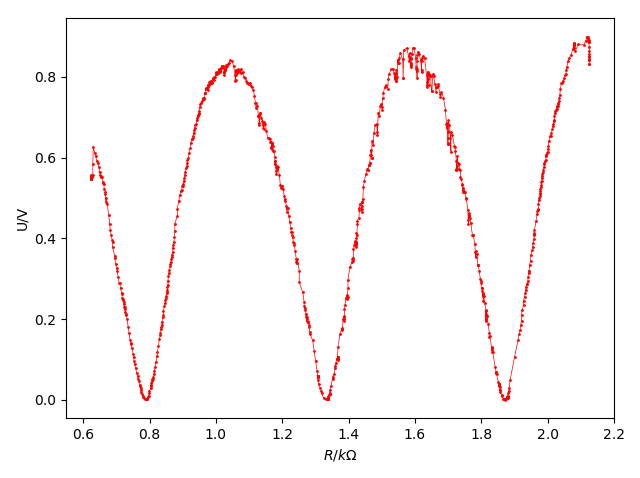
\includegraphics[width=\linewidth]{druckverlauf}
	\caption{Druckverlauf innerhalb Rohres. Zu beachten ist das die Kurve von rechts ausgehend aufgezeichnet wurde.}
	\label{Druckverlauf}
\end{figure}

Der Versuch die Knoten oder Bäuche (Minima bzw. Maxima in Abb. \ref{Druckverlauf}) mithilfe entsprechender Python-Funktionen zu bestimmen lieferte keine zufriedenstellende Ergebnisse.
Da zumindest die Minima sehr scharf abgebildet wurden ist die Bestimmung der Knoten grafisch vorgenommen worden (vgl. Tab.\ref{tab:Druckknoten}). Als Fehler auf die Bestimmung ist der Fehler auf die Widerstandsmessung verwendet worden.

\begin{table}
	\begin{center}
		\begin{tabular}{|c|c|c|}
			\hline 
			n & $R[k\Omega]$ & $\sigma[k\Omega]$ \\ 
			\hline 
			1 & 0.788  & 0.006 \\ 
			\hline 
			2 & 1.344  & 0.006 \\ 
			\hline 
			3 & 1.872 & 0.006 \\ 
			\hline 
		\end{tabular}
		\caption[Druckknoten]{Knoten des Druckverlaufs}
		\label{tab:Druckknoten}
	\end{center}
\end{table}

Eine lineare Regression ($R(n)=a \cdot n+b$) ergibt $a=0.542k\Omega$, $\sigma_{a}=0.004k\Omega$, $b=0.251k\Omega$ und $\sigma_b=0.009k\Omega$. Eine grafische Darstellung findet sich in Abb. \ref{fig:Regression Druckverlauf}.\\
Für diese Anpassung erhält man $\chi^2/ndof=3.630$. Das spricht dafür das der Fehler auf die Knotenbestimmung zu gering abgeschätzt wurde.

\begin{figure}
	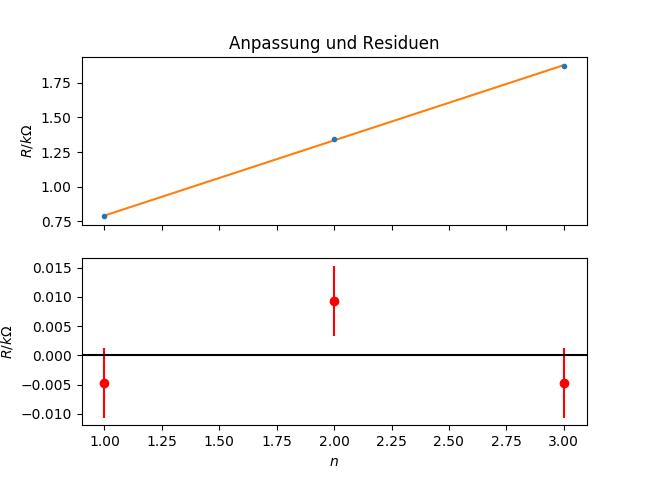
\includegraphics[width=\linewidth]{fitdruckknoten}
	\caption[Regression Knoten]{Regressionsergebnis (oben) und Residuen (unten)}
	\label{fig:Regression Druckverlauf}
\end{figure}

Mit der Steigung der Regression und dem Kalibrierungsfaktor $K=15.97 cm/k\Omega$ des Potentiometers ergibt sich für die Wellenlänge:
\begin{equation}
\lambda=2Ka=17.31cm
\end{equation}
Mit der eingestellten Frequenz von $f=2017.0Hz$ erhält man für die Schallgeschwindigkeit:
\begin{equation}
v=f \lambda = 349.14m/s
\end{equation}

Für die Frequenz wird ein Digitalisierungsfehler von $\sigma_f=0.3Hz$ angenommen($f$ gleichverteilt zwischen $2016.5-2017.5$). Der Fehler auf die Wellenlänge ist damit gegeben durch:
\begin{equation}
\sigma_{\lambda}=2K \sigma_a=0.13cm
\end{equation}
Für den statistischen Fehler der Schallgeschwindigkeit folgt dementsprechend:
\begin{equation}
\sigma_{v,stat.}=v \cdot \sqrt{(\frac{\sigma_{\lambda}}{\lambda})^2+(\frac{\sigma_f}{f})^2}=2.63m/s
\end{equation}

Der systematische Fehler ist durch den Fehler auf die Kalibrierung bedingt. Man erhält mit $\sigma_K=0.07cm/k\Omega$:
\begin{equation}
\sigma_{\lambda,syst.}=2a \sigma_K=0.08cm \quad \Rightarrow \quad \sigma_{v,syst.}=f \sigma_{\lambda,syst.}=1.61m/s
\end{equation}

Insgesamt ergibt sich damit:
\begin{equation}
v=(349.14 \pm 2.63(stat.) \pm 1.61(syst.))m/s
\end{equation}

Dem gegenüber steht der theoretische Wert mit $v_{Theorie}=346.23m/s$. Der gemessene Wert stimmt aufgrund der relativ großen Unsicherheiten relativ gut mit diesem überein.














\part{Schallgeschwindigkeit in Festkörpern}
\section{Schallgeschwindigkeit in Metall}
\subsection{Versuchsbeschreibung}
Der Elastizitätsmodul ist eine Materialkonstante, die in vielen Bereichen, wie beispielsweise in der Bauphysik, eine wichtige Rolle spielt. Er charakterisiert die relative Längenausdehnung in Abhängigkeit von der angreifenden Zugspannung.
\begin{equation}
E = \dfrac{F/A}{\Delta L/L}
\end{equation}
Da der Elastizitätsmodul für Metall (Größenordnung $10^{11} \dfrac{N}{m^2}$) sehr groß ist, lässt er sich nur für dünne Drähte statisch messen. Für Metallstäbe lässt er sich allerdings über die Mesung der Schallgeschwindigkeit mit Hilfe des Zusammenhangs 
\begin{equation}
v_l = \sqrt{\dfrac{E}{\rho}}
\label{eq:001}
\end{equation}
bestimmen. Ein in der Mitte zwischen zwei Punkten eingespannter Stab der Länge L, Masse M und mit Durchmesser D wird durch geeignetes Anschlagen zu longitudinalen Schwingungen angeregt, wobei für die Grundschwingung $\lambda_0 = 2L$ gilt. Mit der Messung der Frequenz $f_0$ berechnet sich die Schallgeschwindigkeit im Metallstab zu
\begin{equation}
v_l = \lambda_0 \cdot f_0
\label{eq:002}
\end{equation}
und der Elastizitätsmodul zu
\begin{equation}
E = 16 f_0^2 \cdot \dfrac{L M}{\pi D^2}.
\label{eq:003}
\end{equation}
\subsection{Versuchsaufbau}
\begin{figure}
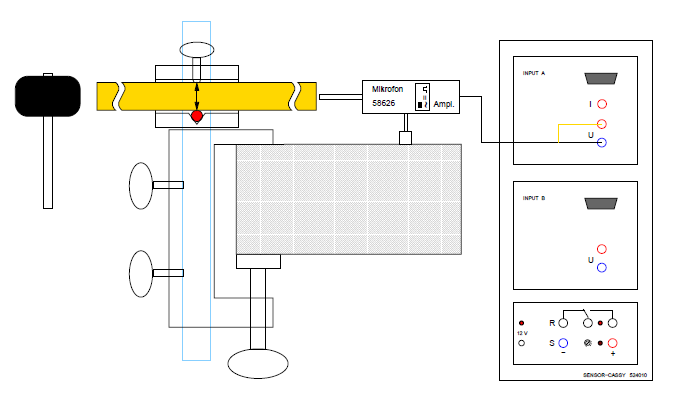
\includegraphics[scale=1]{Bilder/AufbauMessungSchallgeschwindigkeitMetallstab.PNG}
\centering
\caption{Messaufbau Schallgeschwindigkeit in Metallstäben}
\label{StabAufbau}
\end{figure}
Abbildung \ref{StabAufbau} zeigt den mechanischen Aufbau: Der Stab wird mittels einer Kreuzmuffe und einer kurzen Metallstange an einer Tischklemme eingeklemmt. Ein kleiner kurzer Metallstift wird so in die Kreuzmuffe gelegt, dass der Stab nur an zwei gegenüberliegenden Punkten eingeklemmt wird, nämlich zwischen dem Metallstift und der Feststellschraube. Als Messgerät dient ein Mikrofon, welches in ca. 5mm Abstand auf ein Ende des Stabes gerichtet angebracht und an das CASSY angeschlossen wird. 
\subsection{Versuchsdurchführung}
Zunächst müssen die Einstellungen des CASSY angepasst werden. Da die Frequenz der Schwingung bestimmt werden soll, muss die automatische Aufzeichnung verwendet werden. Anhand von Gleichung \eqref{eq:001} lässt sich ersehen, dass die erwarteten Frequenzen sehr hoch sind, daher muss die Intervallzeit im Mikrosekundenbereich ($50 \mu s$) liegen; bei 16000 Messungen liegt die Messdauer dann bei 0,8s. Der Messbereich am CASSY ist nur bedingt relevant, weil sich die Amplitude auch am Mikrofon einstellen lässt. Um Nebeneffekte zu vermeiden, empfiehlt es sich, am CASSY einen mittleren Bereich zu wählen ($|U| \leq 3V$), weil dann auch am Mikrofon ein mittlerer Wert für die Ausgangsamplitude gewählt werden kann. \\

Der Metallstab wird dann mit einem Gummihammer an dem dem Mikrofon abgewandten Ende so angeschlagen, dass die Hammerfläche möglichst parallel zur Stababschlussfläche ist und der Hammerkopf im Moment des Auftreffens nur eine Geschwindigkeitskomponente entlang des Stabes hat. Nach einer sehr kurzen Zeit (Größenordnung 1ms) wird die Messung gestartet. Dadurch wird der Einschwingvorgang in der Messung ignoriert. Dieser Vorgang wird für jeden Stab fünfmal wiederholt. \\

Zuletzt wird der Metallstab ausgemessen und gewogen:
\begin{enumerate}
\item Die Länge L mit dem Bandmaß,
\item den Durchmesser D mit der Mikrometerschraube, gemittelt über fünf Positionen in unterschiedlichen Orientierungen und 
\item die Masse M mit der Analysewaage in drei verschiedenen Orientierungen des Stabes im Raum (Position und Orientierung der Waage bleibt gleich).
\end{enumerate}
\subsection{Versuchsauswertung}
\subsubsection{Rohdaten}
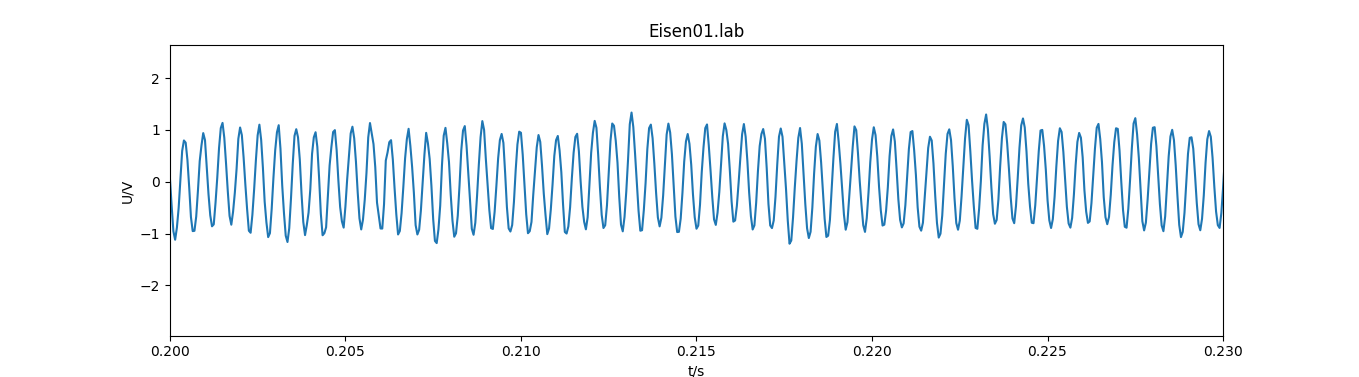
\includegraphics[width=\linewidth,height=\textheight,keepaspectratio]{Bilder/Eisen01.png}
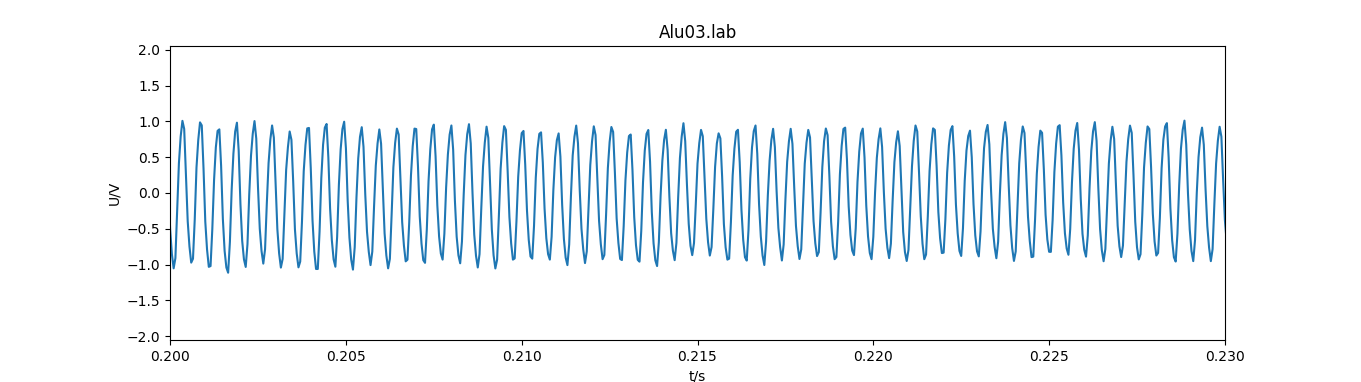
\includegraphics[width=\linewidth,height=\textheight,keepaspectratio]{Bilder/Alu03.png}
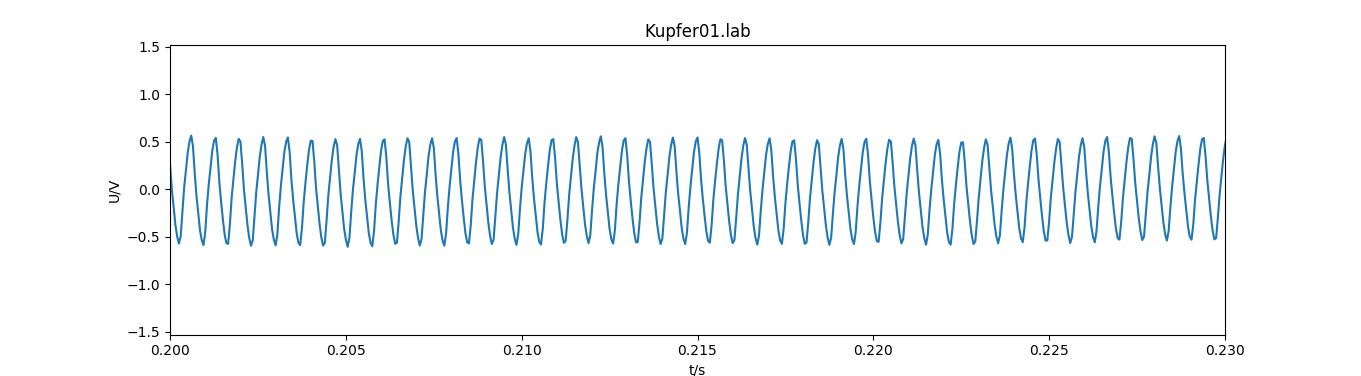
\includegraphics[width=\linewidth,height=\textheight,keepaspectratio]{Bilder/Kupfer01.png}
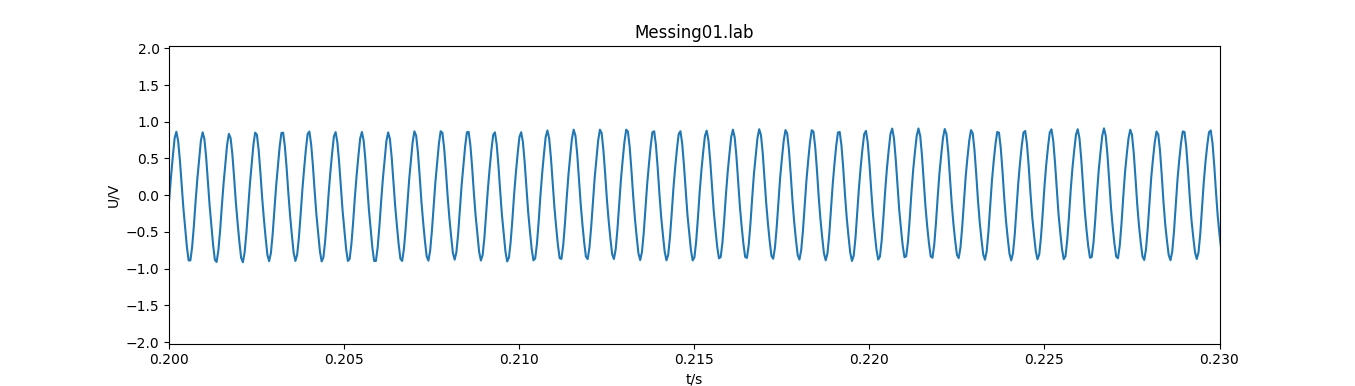
\includegraphics[width=\linewidth,height=\textheight,keepaspectratio]{Bilder/Messing01.png}
\newpage
\subsubsection{Frequenzspektren}
Die Daten wurden mit einer Fast-Fourier-Transformation ausgewertet, da eine normale Fourier-Transformation bei den vorhandenen 20 Datensätzen zu lange gedauert hätte.
Stichproben einer normalen Fourier-Transformation haben aber gezeigt, dass die beiden Methoden nahezu identische Werte ergeben.
Des weiteren wäre eine Bestimmung der Peaklage durch abzählen wegen der hohen Frequenz zu ungenau.\\

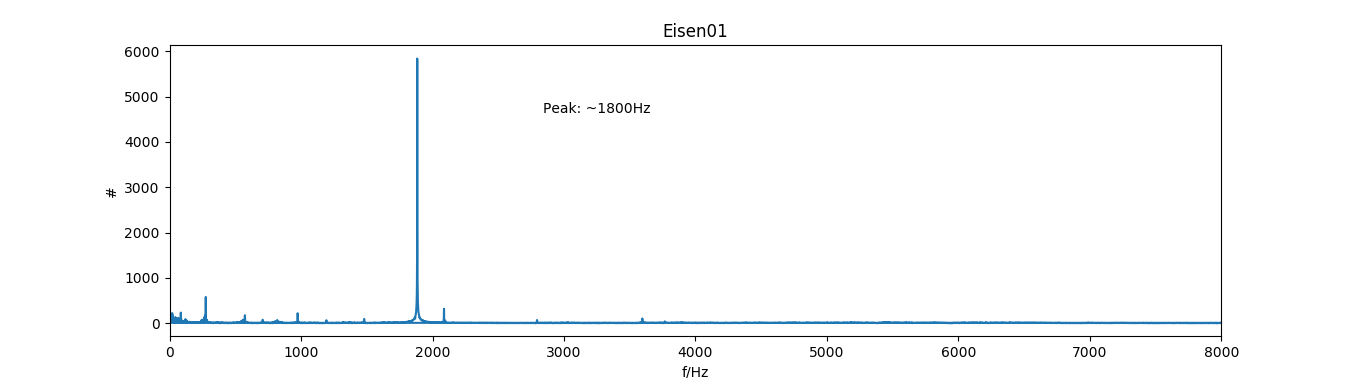
\includegraphics[width=\linewidth,height=\textheight,keepaspectratio]{Bilder/Eisen01_fourier.png}\\
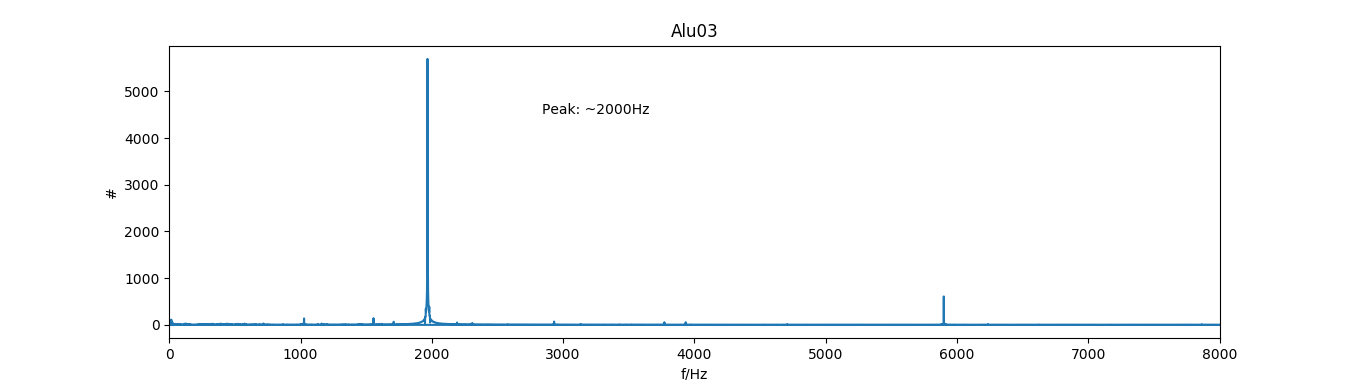
\includegraphics[width=\linewidth,height=\textheight,keepaspectratio]{Bilder/Alu03_fourier.png}\\
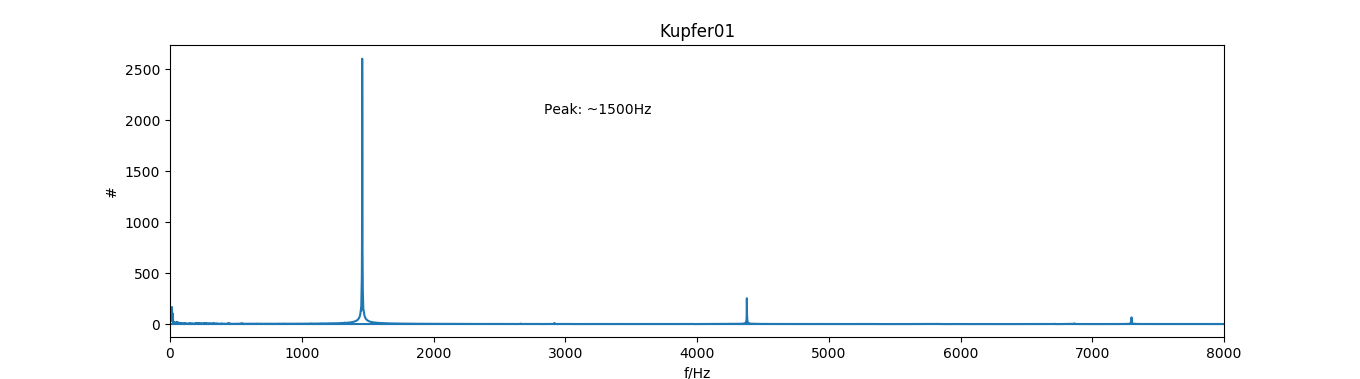
\includegraphics[width=\linewidth,height=\textheight,keepaspectratio]{Bilder/Kupfer01_fourier.png}\\
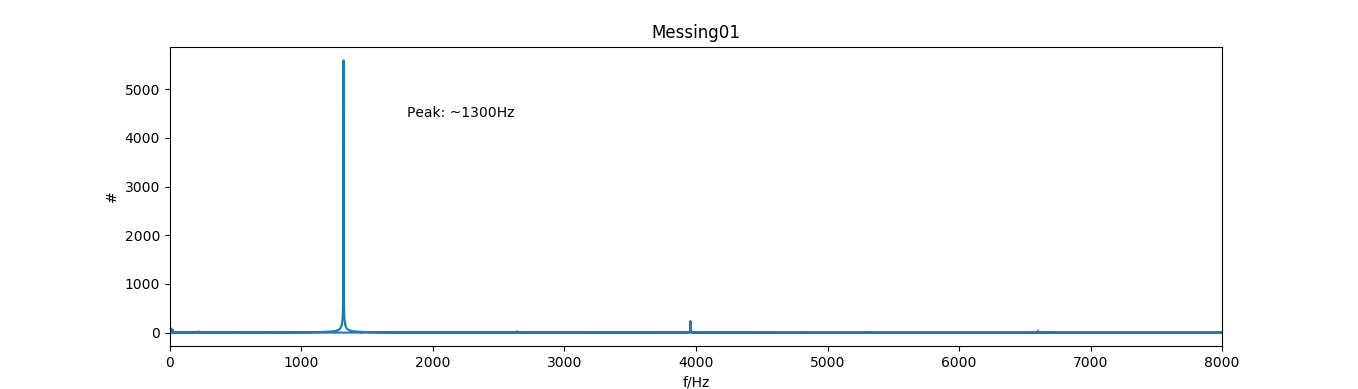
\includegraphics[width=\linewidth,height=\textheight,keepaspectratio]{Bilder/Messing01_fourier.png}\\
Frequenzspektren(von oben nach unten):1.Eisen(Peak:~1800Hz), 2.Aluminium(Peak:~2000Hz), 3.Kupfer(Peak:~1500Hz), 4.Messing(Peak:~1300Hz)
\newpage
\subsubsection{Analyse}
Wegen den Materialeigenschaften der Metalle wir angenommen, dass es sich um Eisen, Aluminium, Kupfer und Messing handelt.
\subsubsection{Ausmessungen}
\begin{tabular}{|c|c|c|c|}
\hline 
Material & Länge[m] & Durchmesser[m] & Masse[kg] \\ 
\hline 
Eisen & $1.303\pm0.0003\pm0.00056$ & $0.01204\pm4.8\cdot10^-5$ & $1.1570\pm1.7\cdot10^-4$ \\ 
\hline 
Aluminium & $1.300\pm0.0003\pm0.00056$ & $0.01199\pm6\cdot10^-5$ & $0.4070\pm6.7\cdot10^-5$ \\ 
\hline 
Kupfer & $1.300\pm0.0003\pm0.00056$ & $0.01195\pm1.8\cdot10^-5$ & $1.2942\pm8.8\cdot10^-5$ \\ 
\hline 
Messing & $1.299\pm0.0003\pm0.00056$ & $0.0119\pm3.7\cdot10^-5$ & $1.2328\pm3.3\cdot10^-5$ \\ 
\hline 
\end{tabular}\\\\
Der statistische Fehler der Länge L ist standardverteilt und beträgt $\sigma_{stat}=\frac{1}{\sqrt{12}}\approx0.3$mm.\\
Der Systematische Fehler ist durch das Maßband mit $0.3+0.2\cdot L$ gegeben. Der Unterschied bei den gemessenen Längen ist minimal, weswegen verallgemeinert $L=1.3m$ und damit $\sigma_{sys}=0.56$mm angegeben wird.\\
Alle anderen Fehler wurden durch Mehrfachmessung aus dem Mittelwert ermittelt.\\
\subsubsection{Ergebnisse der Fourieranalysen}
\begin{tabular}{|c|c|c|c|c|}
\hline 
Material & Eisen & Aluminium & Kupfer & Messing \\ 
\hline 
1.Messung[Hz] & 1883.95 & 1967.00 & 1459.67 & 1321.40 \\ 
\hline 
2.Messung[Hz] & 1884.01 & 1966.96 & 1459.45 & 1321.41 \\ 
\hline 
3.Messung[Hz] & 1884.02 & 1966.93 & 1459.17 & 1321.40 \\ 
\hline 
4.Messung[Hz] & 1884.03 & 1966.60 & 1459.47 & 1321.41 \\ 
\hline 
5.Messung[Hz] & 1884.03 & 1966.58 & 1459.46 & 1321.41 \\ 
\hline 
\end{tabular} 
\\
\\
Daraus folgen die Mittelwerte und der Fehler:\\
Eisen: 		($1884.007\pm0.015$)Hz\\
Aluminium:	($1966.813\pm0.092$)Hz\\
Kupfer:		($1459.406\pm0.058$)Hz\\
Messing:	($1321.407\pm0.002$)Hz\\
\\
Daraus kann man mit den Gleichungen (\ref{eq:002}) und (\ref{eq:003}) die Schallgeschwindigkeit v und das E-Modul E berechnen.\\
Für den Fehler auf v gilt:
\begin{equation}
\sigma_v= v\cdot\sqrt{(\frac{\sigma_L}{L})^2+(\frac{\sigma_f}{f})^2}
\end{equation}
Für den Fehler auf f gilt:
\begin{equation}
\sigma_f=f\cdot\sqrt{(\frac{\sigma_L}{L})^2+2\cdot(\frac{\sigma_f}{f})^2+(\frac{\sigma_M}{M})^2+2\cdot(\frac{\sigma_D}{D})^2}
\end{equation}
\begin{tabular}{|c|c|c|c|}
\hline 
Material  & Frequenz[Hz] & Geschwindigkeit[m/s] & E-Modul[GPa] \\ 
\hline 
Eisen & $1884.007\pm0.015$ & $4909.7\pm1.1\pm2.1$ & $188.0\pm1.1$ \\ 
\hline 
Aluminium & $1966.813\pm0.092$ & $5113.7\pm1.2\pm2.2$ & $72.5\pm0.5$ \\ 
\hline 
Kupfer & $1459.406\pm0.058$ & $3794.5\pm0.9\pm1.6$ & $127.7\pm0.3$ \\ 
\hline 
Messing & $1321.407\pm0.002$ & $3433.0\pm0.8\pm1.5$ & $100.5\pm0.4$ \\ 
\hline 
\end{tabular} 
\\
Hinweis: Die systematische Abweichung auf das E-Modul ist immer kleiner als 0.05 und damit für die Messwerte unwichtig
\newpage
\subsubsection{Vergleich mit Literaturwerten}
Die Literaturwerte sind im allgemeinen für eine Temperatur von 20C angegeben. Die Umgebungstemperatur lag bei 24C. Dieser Unterschied auf die Endwerte ist aber für Festkörper vernachlässigbar.
\begin{table}
\begin{tabular}{|c|c|c|}
\hline 
Material & gemessene Geschw.[m/s] & Literaturwert[m/s] \\ 
\hline 
Eisen & $4909.7\pm3.2$ & 4910-5170  \\ 
\hline 
Aluminium & $5113.7\pm3.4$ & 5350-6250  \\ 
\hline 
Kupfer & $3794.5\pm2.5$ & 4660 \\ 
\hline 
Messing & $3433.0\pm2.3$ & 3500 \\ 
\hline 
\end{tabular} 
\begin{tabular}{|c|c|c|}
\hline 
Material & gemessenes E-Modul[GPa] & Literaturwert[GPa] \\ 
\hline 
Eisen & $188.0\pm1.1$ & 180-210 \\ 
\hline 
Aluminium & $72.5\pm0.5$ & 70 \\ 
\hline 
Kupfer & $127.7\pm0.3$ & 100-130 \\ 
\hline 
Messing & $100.5\pm0.4$ & 78-123 \\ 
\hline 
\end{tabular} 
\caption{Gemessene Daten und Literaturwerte}
Anmerkung: Für den Wert des E-Moduls von Eisen wurde wegen fehlender Quellen das von Stahl genommen.
\end{table}
\paragraph{Eisen}
Der gemessene Wert für die Geschwindigkeit liegt im Rahmen von einer Standardabweichung im Bereich des Literaturwertes.
Das Elastizitätsmodul stimmt ebenfalls mit dem Literaturwert überein.
\paragraph{Aluminium}
Hier ist die gemessene Geschwindigkeit um 236m/s(70 Standardabweichungen)kleiner als der Literaturwert, das Elastizitätsmodul allerdings um 2.5GPa(5 Standardabweichungen größer)
\paragraph{Kupfer}
Die Geschwindigkeit weicht hier sogar um 866m/s(347 Standardabweichungen) vom Literaturwert ab. Gleichzeitig liegt aber das Elastizitätsmodul im angegebenen Bereich.
\paragraph{Messing}
Die gemessene Geschwindigkeit ist um 67m/s(30 Standardabweichungen) zu klein.
Das Elastizitätsmodul liegt aber wieder im Literatur angegebenen Bereich.
\\\\
Offenbar liegt vor allem bei Aluminium und Kupfer ein sehr großer unbekannter Fehler bei der Geschwindigkeit vor. Es besteht die Möglichkeit, dass die Literaturangaben andere Materialeigenschaften voraussetzen, da die Werte für das Elastizitätsmodul trotz dieses großen Fehlers richtig sind
\newpage


\section{Akustik der Gitarre}
\subsection{Versuchsbeschreibung}
Die Überlagerung zweier Wellen kann mit dem Superpositionsprinzip
\begin{equation}
A(x = 0, t) = \sum_{n=1}^N A_n \cdot \sin (w_nt) \cdot \cos (k_nx) = \sum_{n=1}^N A_n \cdot \sin (w_nt)
\end{equation}
beschrieben werden. Wendet man dieses auf zwei Wellen mit gleicher Amplitude an, lässt sich das Ergebnis mithilfe der Additionstheoreme in einen Term der Form
\begin{equation}
A(x = 0, t) = A_0 \cdot \sin (w_st) \cdot \sin (w_{res}t)
\end{equation}
mit
\begin{equation}
w_s = \dfrac{w_1 - w_2}{2} \quad und \quad w_{res} = \dfrac{w_1 + w_2}{2}
\label{eq:Schwebungsfrequenz}
\end{equation}
umformen. Das wird als Schwebung bezeichnet. Wie sich unschwer erkennen lässt, ist der Schwebungseffekt nur dann hörbar, wenn die beiden ursprünglichen Frequenzen nah beieinander liegen, denn nur dann gilt $w_s \ll w_{res}$. \\
Bei einer Gitarre lässt sich der Ton einer Leersaite mit der nächsthöheren Saite durch Anschlagen bei Verkürzen der Saite am fünften Bund reproduzieren. Wenn nun eine der beiden Saiten leicht verstimmt ist, tritt die Schwebung gut hörbar auf.
\subsection{Versuchsaufbau}
\begin{figure}
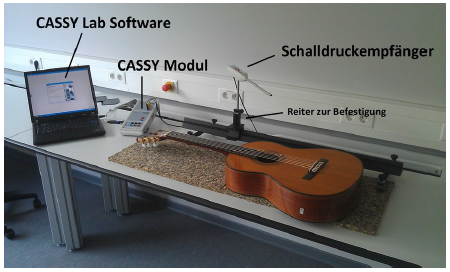
\includegraphics[scale=1]{Bilder/AufbauAkustikGitarre.PNG}
\centering
\caption{Messaufbau Schallgeschwindigkeit in Metallstäben}
\label{GitarreAufbau}
\end{figure}
Die Gitarre wird auf einer dämpfenden Unterlage aufgelegt, um äußere Einflüsse zu minimieren. Das Mikrofon wird in einem Abstand von ca. 25cm über dem Schallloch der Gitarre befestigt und an das CASSY angeschlossen.
\subsection{Versuchsdurchführung}
\label{GitarreEinstellungen}
Zunächst muss die Gitarre gestimmt werden. Dazu wird das Stimmgerät am Gitarrenkopf befestigt und eine Saite unverkürzt angeschlagen. Das Stimmgerät zeigt die ggfs. notwendige Änderung der Saitenspannung an. Dies wird mit allen Saiten wiederholt. Nun wird eine Saite verstimmt. Dazu wird die Saitenspannung um eine halbe Umdrehung der Spannschraube verändert. Der Messbereich am CASSY bleibt im Vergleich zum ersten Versuch unverändert bei $|U| \leq 3V$. Da die Frequenzen einer Gitarre nicht ganz so hoch liegen reicht hier ein Messintervall von $200 \mu s$; bei 16000 Messungen ergibt sich eine Messdauer von 3,2s. \\
Es werden für die Messung immer jeweils die verstimmte Saite am fünften Bund verkürzt und die nächsthöhere Saite angeschlagen. Die Messung wird auch hier wieder mit kurzem Zeitversatz (ca. 20ms) gestartet, um den Einschwingvorgang in der Messung zu ignorieren. Dieser Vorgang wird fünfmal wiederholt.

\subsection{Versuchsauswertung}
\subsubsection{Rohdaten}
\begin{figure}
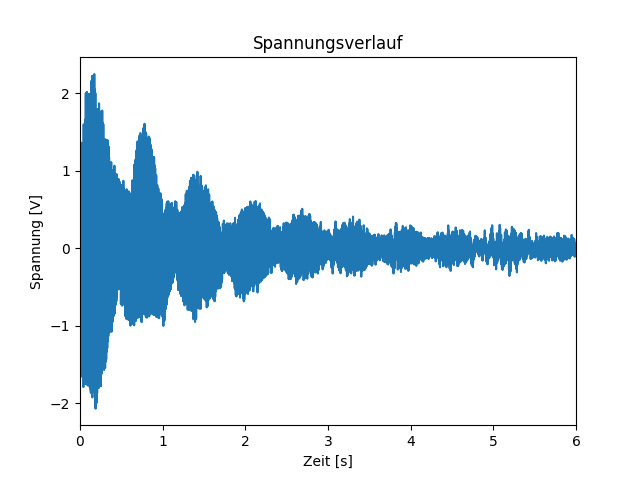
\includegraphics[scale=1]{Bilder/Schwebung_roh.png}
\centering
\caption{Schwingung zweier Gitarrensaite mit nur leicht unterschiedlichen Frequenzen}
\label{Schwebung_roh}
\end{figure}
Die Schwebung ist gut durch die Schwankungen der Amplitude zu erkennen. Die resultierende Frequenz ist nicht direkt ersichtlich, dazu muss in das Bild "reingezoomt" werden. Dabei gerät die Schwebung aus dem Blickfeld.
\begin{figure}
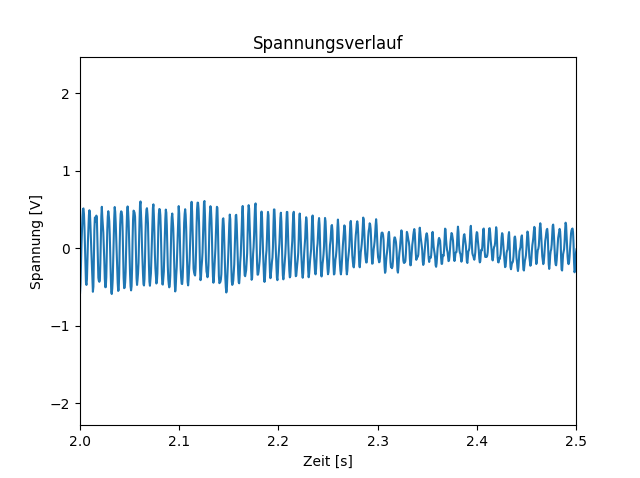
\includegraphics[scale=1]{Bilder/Schwebung_reingezoomt.png}
\centering
\caption{Schwingung zweier Gitarrensaite mit nur leicht unterschiedlichen Frequenzen; kurzes Zeitintervall}
\label{Schwebung_zoom}
\end{figure}
\subsubsection{Frequenzspektren}
Die Schwebungsfrequenz kann nun auf zweierlei Arten bestimmt werden. Möglichkeit eins ist die Berechnung aus den beiden Originalfrequenzen, die mithilfe der Fast-Fourier-Transformation aus den Daten bestimmt werden. Diese liefert für jeden Datensatz ein Frequenzspektrum wie in Abbildung \ref{Schwebung_Frequenzspektrum}. Die Schwebungsfrequenz wird dann mit Gleichung \ref{eq:Schwebungsfrequenz} berechnet. \\
Die zweite Möglichkeit besteht darin, die Schwebungsfrequenz durch Abzählen der Amplitudenminima in den Rohdaten zu bestimmen. Dazu werden alle sichtbaren Amplitudenminima abgezählt und anschließend durch die Differenz der Zeitpunkte des ersten und des letzten Minimums geteilt.
\begin{figure}
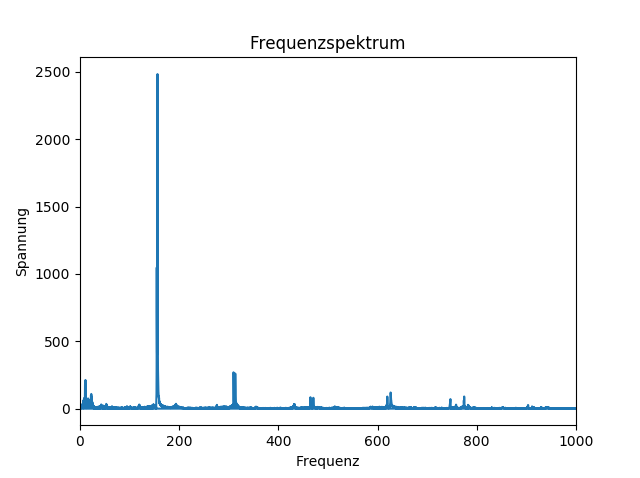
\includegraphics[scale=1]{Bilder/Frequenzspektrum_ges.png}
\centering
\caption{Gesamtes Frequenzspektrum}
\label{Schwebung_Frequenzspektrum}
\end{figure}
Der erste hohe Peak ist zweigeteilt, wie sich bei näherer Betrachtung gut erkennen lässt. Das sind die beiden Saitenfrequenzen (vergleiche Abbildung \ref{Schwebung_zoom}).
\begin{figure}
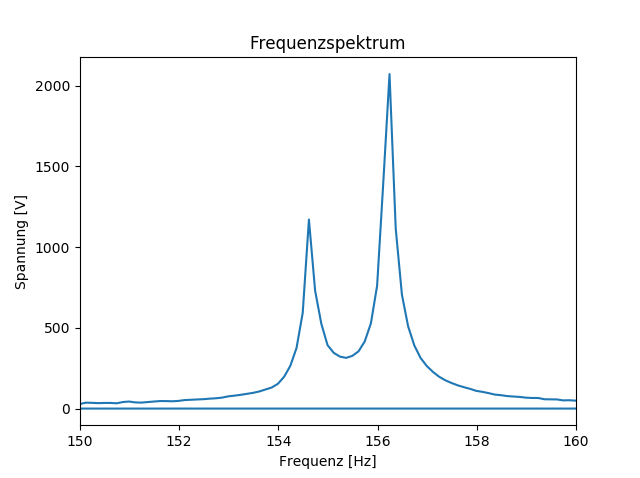
\includegraphics[scale=1]{Bilder/Frequenzspektrum_zoom.png}
\centering
\caption{Ausgeschnittenes Frequenzspektrum}
\label{Schwebung_Frequenzspektrum_zoom}
\end{figure}
\subsubsection{Analyse}
Die beiden beschriebenen Methoden führen zu folgenden Ergebnissen: \\
\begin{tabular}{|c|c|c|}
\hline 
• & Ergebnis der FFT & Wert durch Ablesen \\ 
\hline 
1. Messung & (1.06 $\pm$ 0.36) Hz & (1.60 $\pm$ 0.10) Hz \\ 
\hline 
2. Messung & (1.25 $\pm$ 0.07) Hz & (1.64 $\pm$ 0.10) Hz \\ 
\hline 
3. Messung & (1.75 $\pm$ 0.14) Hz & (1.85 $\pm$ 0.10) Hz \\ 
\hline 
4. Messung & (1.25 $\pm$ 0.14) Hz & (1.61 $\pm$ 0.10) Hz \\ 
\hline 
5. Messung & (1.31 $\pm$ 0.07) Hz & (1.43 $\pm$ 0.10) Hz \\ 
\hline 
\end{tabular} \\
\\Der Fehler auf die Frequenz aus der FFT ergibt sich dabei aus einer Bestimmung der Peak-Breite und der Annahme, dass die Frequenz innerhalb dieses Peaks gleichverteilt ist. Damit berechnet sich dieser für eine Peak-Breite $bp_1$ auf die erste und eine Peak-Breite $bp_2$ auf die zweite Frequenz zu
\begin{equation}
\sigma_f = \dfrac{bp_1 + bp_2}{\sqrt{12}}
\end{equation}
\subsubsection{Auswertung}
Die Ergebnisse aus der FFT und die abgelesenen Werte liegen jeweils zwischen weniger als 1 und knappen 6 Standardabweichungen (aus der FFT) auseinander. Auffällig ist, dass die Werte aus der FFT alle kleiner sind, als die zugehörigen abgelesenen Werte.
\section{Bestimmung der Saitenspannung einer Gitarre}
\subsection{Versuchsbeschreibung}
Eine für die Tonqualität wichtige Eigenschaft einer Saite ist das Verhältnis aus Saitenspannung T zu Massebelag $\mu$. Es gilt der Zusammenhang
\begin{equation}
f_n = \dfrac{n}{2L} \cdot \sqrt{\dfrac{T}{\mu}}.
\label{eq:SpannungMassebelag}
\end{equation}
Dabei ist L die Länger der am Bund verkürzten, frei schwingenden Saite und n charakterisiert, um welche (Ober-)Schwingung es sich handelt. Der Grundton ergibt sich also für $n=1$.
\subsection{Versuchsaufbau}
Der Versuchsaufbau ist identisch zu dem im Kapitel \ref{GitarreAufbau} beschriebenen.
\subsection{Versuchsdurchführung}
Zunächst müssen die Längen der an den Bünden verkürzten Saiten mit dem Maßband gemessen werden. \\
Die Messparameter für Mikrofon und CASSY sind identisch wie in Kapitel \ref{GitarreEinstellungen} beschrieben.
Anschließend wird die Saite angeschlagen und die Messung mit kurzem Zeitversatz (ca. 20ms) gestartet. Diese Messung wird zehnmal wiederholt, wobei jedes Mal die Saite um einen Bund verkürzt wird.
\subsection{Versuchsauswertung}
\subsubsection{Rohdaten}
\begin{figure}
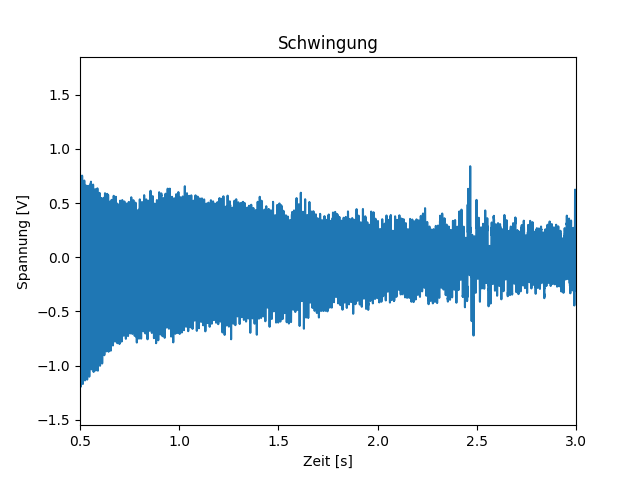
\includegraphics[scale=1]{Bilder/Gitarre_Schwingung.png}
\centering
\caption{Frequenzspektrum einer Gitarrensaite}
\label{Schwingung_Rohdaten}
\end{figure}
Abbildung \ref{Schwingung_Rohdaten} zeigt die Rohdaten. Hieraus lässt sich kaum etwas ablesen, abgesehen davon, dass es sich um eine Schwingung handelt.
\subsubsection{Frequenzspektren}
Wesentlich mehr Aufschluss gibt da das Frequenzspektrum aus der FFT (siehe Abbildung \ref{Saite_Frequenzspektrum}). Hier sind die Grundschwingung (erster Peak) und die Oberschwingungen gut erkennbar, ebenso wie das Abfallen der Amplituden der Peaks mit $A_n \propto \dfrac{1}{n}$.
\begin{figure}
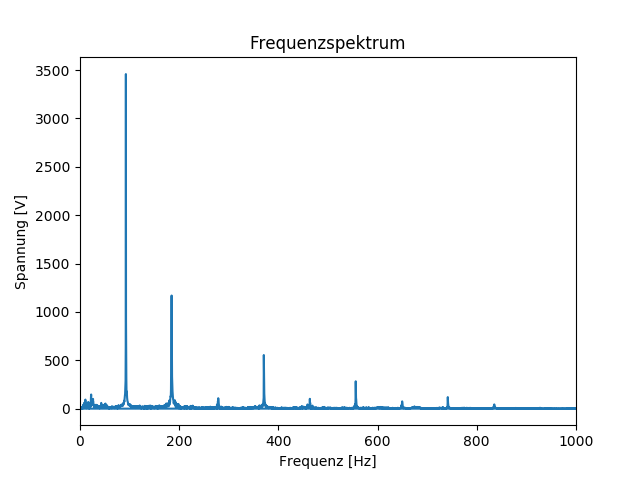
\includegraphics[scale=1]{Bilder/FrequenzspektrumGitarrensaite.png}
\centering
\caption{Frequenzspektrum einer Gitarrensaite}
\label{Saite_Frequenzspektrum}
\end{figure}
\subsubsection{Analyse}
Die aus den Daten mit der FFT ermittelten Frequenzen und die zuvor an der Gitarre gemessenen Saitenlängen finden sich in der Tabelle. \\
\begin{tabular}{|c|c|c|}
\hline 
Bund & Frequenz [Hz] & Länge [m] \\ 
\hline 
1 & 83,75 $\pm$ 0,09 & 0,650 $\pm$ 0,001 \\ 
\hline 
2 & 87,18 $\pm$ 0,27 & 0,616 $\pm$ 0,001 \\ 
\hline 
3 & 92,18 $\pm$ 0,36 & 0,582 $\pm$ 0,001 \\ 
\hline 
4 & 95,93 $\pm$ 0,09 & 0,548 $\pm$ 0,001 \\ 
\hline 
5 & 103,12 $\pm$ 0,09 & 0,516 $\pm$ 0,001 \\ 
\hline 
6 & 106,24 $\pm$ 0,09 & 0,487 $\pm$ 0,001 \\ 
\hline 
7 & 116,24 $\pm$ 0,72 & 0,459 $\pm$ 0,001 \\ 
\hline 
8 & 122,49 $\pm$ 0,81 & 0,434 $\pm$ 0,001 \\ 
\hline 
9 & 129,37 $\pm$ 0,09 & 0,410 $\pm$ 0,001 \\ 
\hline 
10 & 134,99 $\pm$ 0,09 & 0,387 $\pm$ 0,001 \\ 
\hline 
\end{tabular} 
\\
\begin{figure}
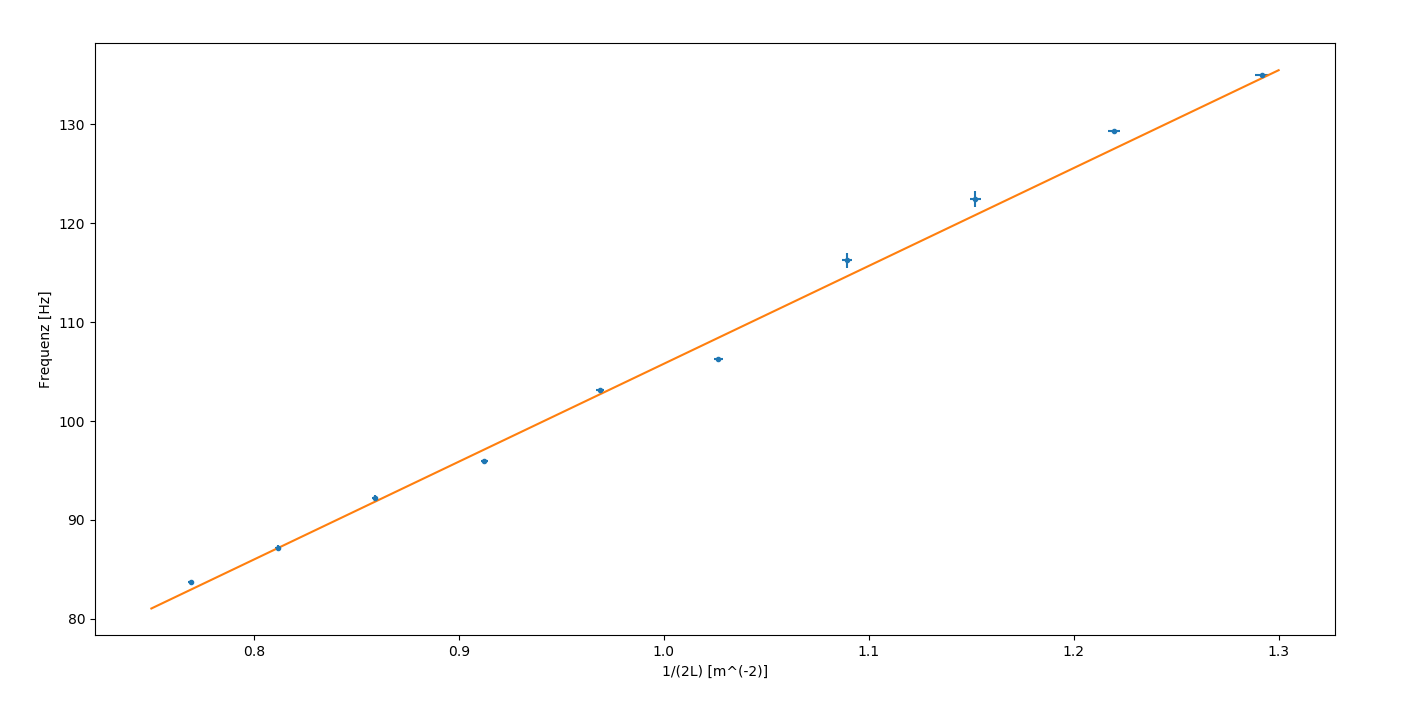
\includegraphics[scale=0.5]{Bilder/SpannungMassebelagLineareRegression.png}
\centering
\caption{Lineare Regession}
\label{LineareRegressionSpannungMassebelag}
\end{figure}
Mittels Gleichung \ref{eq:SpannungMassebelag} lässt sich nun eine lineare Regression durch auftragen von $f$ gegen $\dfrac{1}{2L}$ durchführen (wie in Abbildung \ref{LineareRegressionSpannungMassebelag} gezeigt). Die Steigung der Ausgleichgeraden ist dann die Wurzel aus dem Verhältnis der Saitenspannung zu Massebelag. \\
Führt man dies durch, erhält man folgenden Wert:
\begin{equation}
\sqrt{\dfrac{T}{\mu}} = (98,98 \pm 2,67)\sqrt{\dfrac{Nm}{kg}}
\end{equation}
\subsubsection{Vergleich mit Herstellerangaben}
Der Hersteller hat für die Saite die Werte zu $T = 63,50N$ und $\mu = 5,6712 \cdot 10^{-3} \dfrac{kg}{m}$ angegeben. Damit ergibt sich der "Literaturwert" für die gemessene Größe zu 
\begin{equation}
\sqrt{\dfrac{T}{\mu}} = 105,82 \sqrt{\dfrac{Nm}{kg}}
\end{equation}
Der gemessene Wert liegt also ca. 2,6 Standardabweichungen von den Herstellerangaben entfernt.
\end{document}
